\documentclass[9pt]{beamer}
\usepackage{fontspec}
\usepackage[english,bulgarian]{babel}
\usepackage{xcolor}

\defaultfontfeatures{Ligatures=TeX}
\newfontfamily\cyrillicfont{Comfortaa-Regular}
\newfontfamily\cyrillicfonttt{Comfortaa-Regular}
\newfontfamily\fontcomic[NFSSFamily=roboto]{Roboto}
\setsansfont{Comfortaa-Regular}

\definecolor{mygreen}{rgb}{0.3333, 0.4196, 0.1843}
\definecolor{mypink}{rgb}{0.858, 0.188, 0.478}

\graphicspath{ {./resources/} }

\usetheme{metropolis}
\begin{document}
    \section{Разпознаване на емоции в сигнали от реч и ЕЕГ}
    \begin{frame}{В началото}
        \begin{itemize}
            \item ... бе Словото
            \pause 
            \item Експлицитен и имплицитен канал при общуване
            \pause 
            \item Прозодия (ритъм, интонация, ударение)
        \end{itemize}
        \pause 
        \begin{center}
            
\includegraphics[width=\textwidth]{meaning.png}%

            \footnotesize{Попълването на вица е оставено за упражнение на читателя}
            \normalsize
        \end{center}
        \pause
        \begin{itemize}
            \item Съчетаване на първичен (ЕЕГ) и вторичен (реч) канал
        \end{itemize}        
    \end{frame}
    
    \begin{frame}{Влакче на мисълта}
        \begin{center}
        \begin{itemize}
            \setlength\itemsep{\fill}
            \item[$\triangleright$] Нулева зона (какво е емоция)
            \pause 
            \item[$\triangleright$] Сигнал от реч
            \pause 
            \item[$\triangleright$] Сигнал от ЕЕГ
            \pause 
            \item[$\triangleright$] Съчетаване на двата сигнала
            \pause 
            \item[$\triangleright$] Резултати
            \pause 
            \item[$\triangleright$] Заключение
        \end{itemize}
        \end{center}
    \end{frame}

    \section{Нулета зона (какво е емоция)}
    \begin{frame}{Нулева зона (какво е емоция)}
        \begin{itemize}
            \setlength\itemsep{\fill}
            \item Теорията на Дарвин
            \begin{itemize}
                \pause
                \item[$-$] ``Принцип на полезните навици''
                \pause
                \item[$-$] ``Принцип на противоположностите''
                \pause
                \item[$-$] ``Принцип на нервните сигнали''
            \end{itemize}
            \pause
            \item Продължението на Плутчик (1980)
        \end{itemize}
        \pause
        \begin{quote}
            \textbf{Емоцията е сложна верига от събития, която започва с някакъв стимул.} В следствие настъпва фаза на ``изпитване на емоция'' и фаза на физиологични промени. Те предизвикват целенасочено държание, което цели да премахне дразнението на стимула и да върне състоянието на еквилибриум.
        \end{quote}
    \end{frame}
    \begin{frame}{Нулева зона (какво е емоция)}
        \begin{columns}[T] % align columns
            \begin{column}{.53\textwidth}
                \begin{center}
                    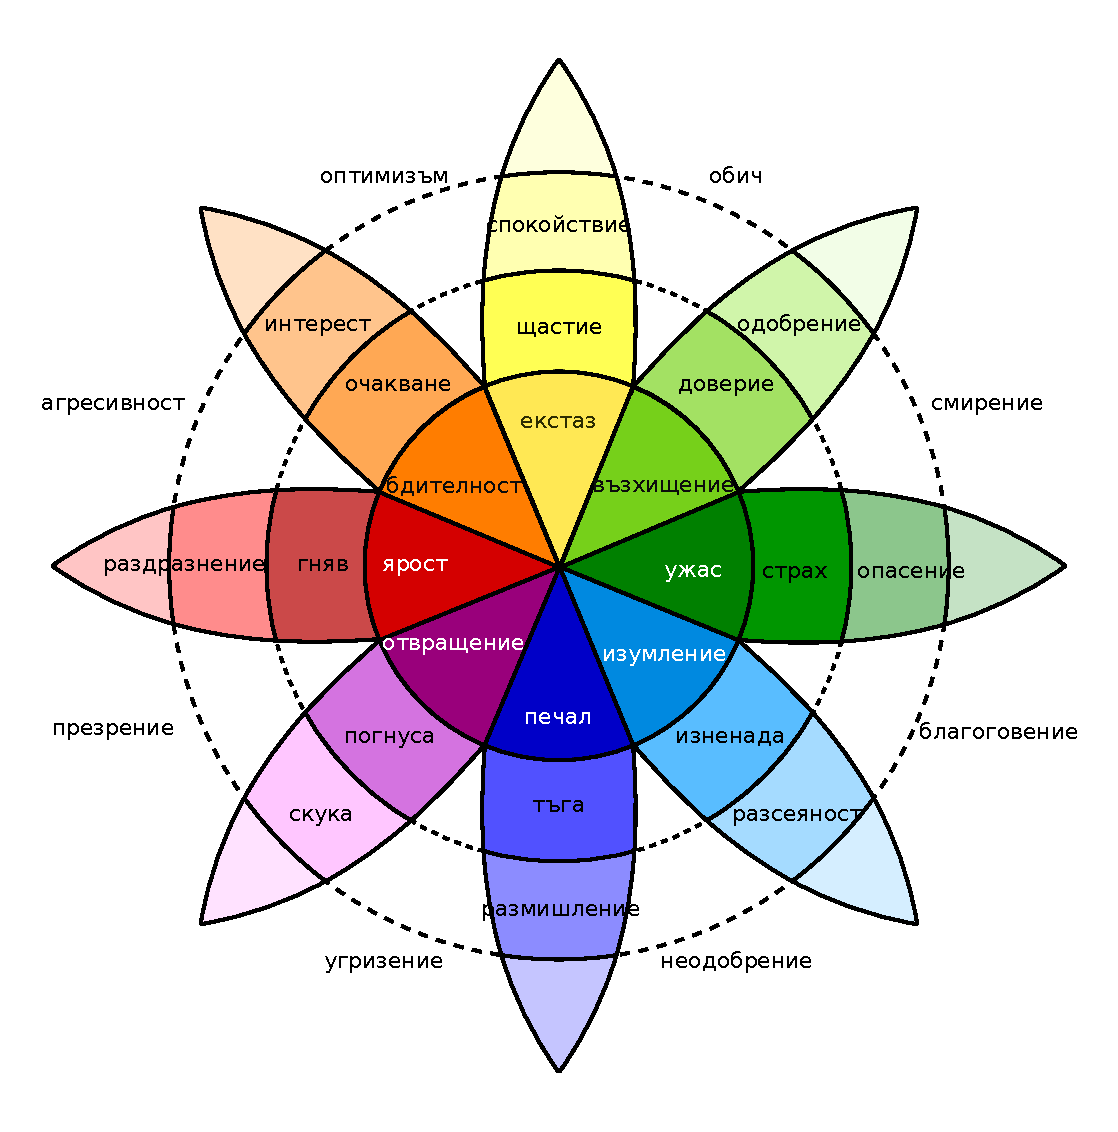
\includegraphics[width=\textwidth]{plutchik}%
                \end{center}
            \end{column}%
            \hfill%
            \pause
            \begin{column}{.45\textwidth}
                \vspace{1cm}
                ${\color{mygreen}+}$ Всяка емоция може да се изрази като комбинация на основните
                
                \vspace{2cm}
                \pause
                ${\color{mypink}-}$ Осем е голямо число
            \end{column}%
        \end{columns}
    \end{frame}
    \setbeamercolor{background canvas}{bg=white}
    \begin{frame}{Нулева зона (какво е емоция)}
        \begin{itemize}
            \item VAD модела - Алберт Мейерабиан и Джеймс Ръсел (1974)
        \end{itemize}
        \pause
        \begin{center}
            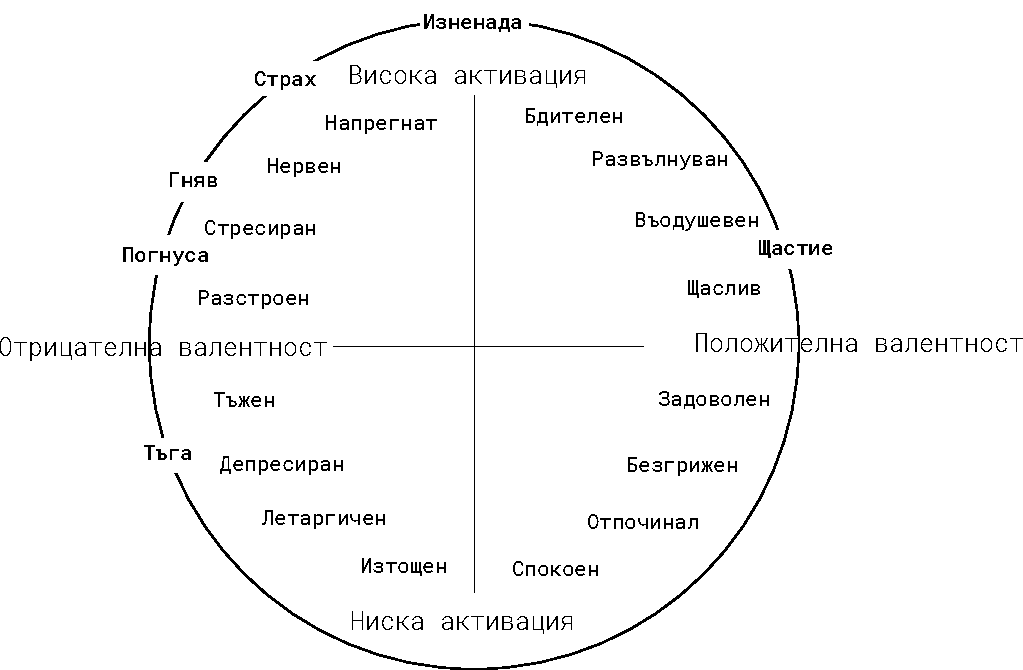
\includegraphics[width=0.9\textwidth]{valence_arousal}%
        \end{center}
        \pause
        \begin{itemize}
            \item В сигнала от реч се измерва по-лесно активацията
            \pause
            \item В сигнала от ЕЕГ се измерва по-лесно валентността
        \end{itemize}
    \end{frame}

    \begin{frame}{Нулева зона (какво е емоция)}
        \begin{columns}[T] % align columns
            \begin{column}{.38\textwidth}
                \textbf{Избрани емоции:}
                \vspace{1cm}\\
                \phantom{$\bullet\ $ Гняв}
                \vspace{1cm}\\
                \phantom{$\bullet\ $ Щастие}
                \vspace{1cm}\\
                \phantom{$\bullet\ $ Неутрална емоция}
                \vspace{1cm}\\
                \phantom{$\bullet\ $ Тъга}
            \end{column}%
            \hfill%
            \begin{column}{.60\textwidth}
                \vspace{1cm}
                \begin{center}
                    
\includegraphics[width=\textwidth]{valence_arousal_empty}%
                \end{center}
            \end{column}%
        \end{columns}
    \end{frame}

    \begin{frame}{Нулева зона (какво е емоция)}
        \begin{columns}[T] % align columns
            \begin{column}{.38\textwidth}
                \textbf{Избрани емоции:}
                \vspace{1cm}\\
                $\bullet\ $ Гняв
                \vspace{1cm}\\
                \phantom{$\bullet\ $ Щастие}
                \vspace{1cm}\\
                \phantom{$\bullet\ $ Неутрална емоция}
                \vspace{1cm}\\
                \phantom{$\bullet\ $ Тъга}
            \end{column}%
            \hfill%
            \begin{column}{.60\textwidth}
                \vspace{1cm}
                \begin{center}
                    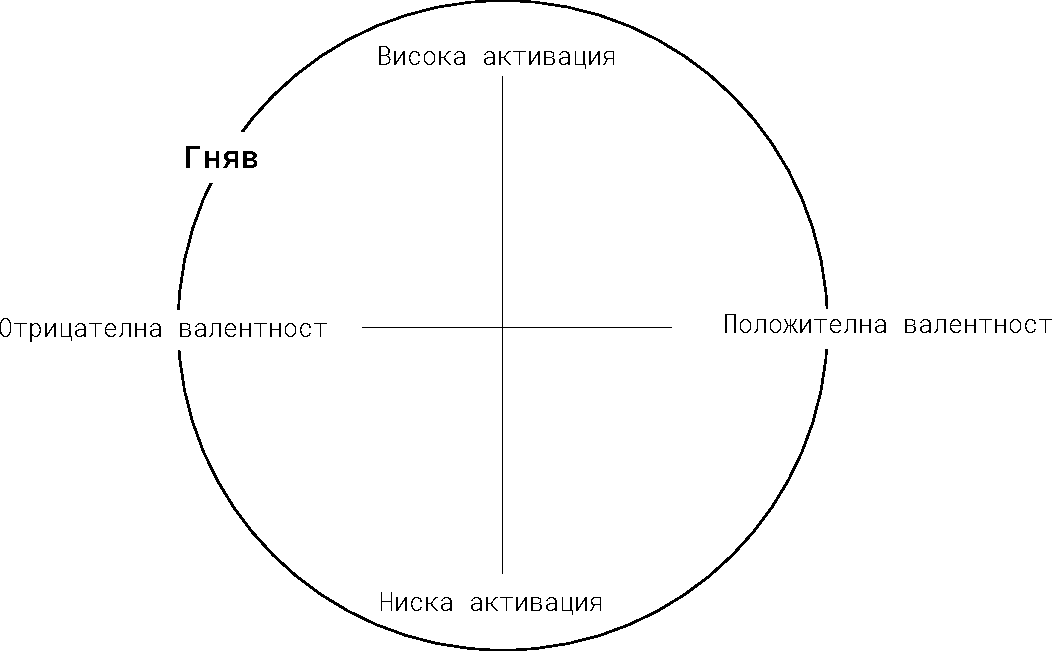
\includegraphics[width=\textwidth]{valence_arousal_a}%
                \end{center}
            \end{column}%
        \end{columns}
    \end{frame}


    \begin{frame}{Нулева зона (какво е емоция)}
        \begin{columns}[T] % align columns
            \begin{column}{.38\textwidth}
                \textbf{Избрани емоции:}
                \vspace{1cm}\\
                $\bullet\ $ Гняв
                \vspace{1cm}\\
                $\bullet\ $ Щастие
                \vspace{1cm}\\
                \phantom{$\bullet\ $ Неутрална емоция}
                \vspace{1cm}\\
                \phantom{$\bullet\ $ Тъга}
            \end{column}%
            \hfill%
            \begin{column}{.60\textwidth}
                \vspace{1cm}
                \begin{center}
                    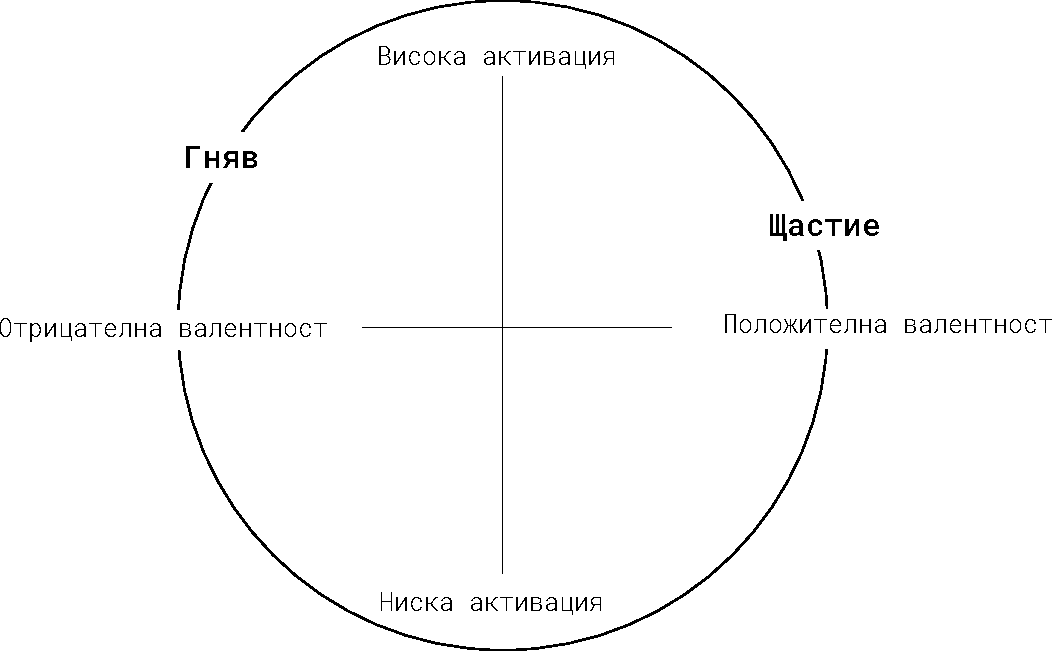
\includegraphics[width=\textwidth]{valence_arousal_ah}%
                \end{center}
            \end{column}%
        \end{columns}
    \end{frame}

    \begin{frame}{Нулева зона (какво е емоция)}
        \begin{columns}[T] % align columns
            \begin{column}{.38\textwidth}
                \textbf{Избрани емоции:}
                \vspace{1cm}\\
                $\bullet\ $ Гняв
                \vspace{1cm}\\
                $\bullet\ $ Щастие
                \vspace{1cm}\\
                $\bullet\ $ Неутрална емоция
                \vspace{1cm}\\
                \phantom{$\bullet\ $ Тъга}
            \end{column}%
            \hfill%
            \begin{column}{.60\textwidth}
                \vspace{1cm}
                \begin{center}
                    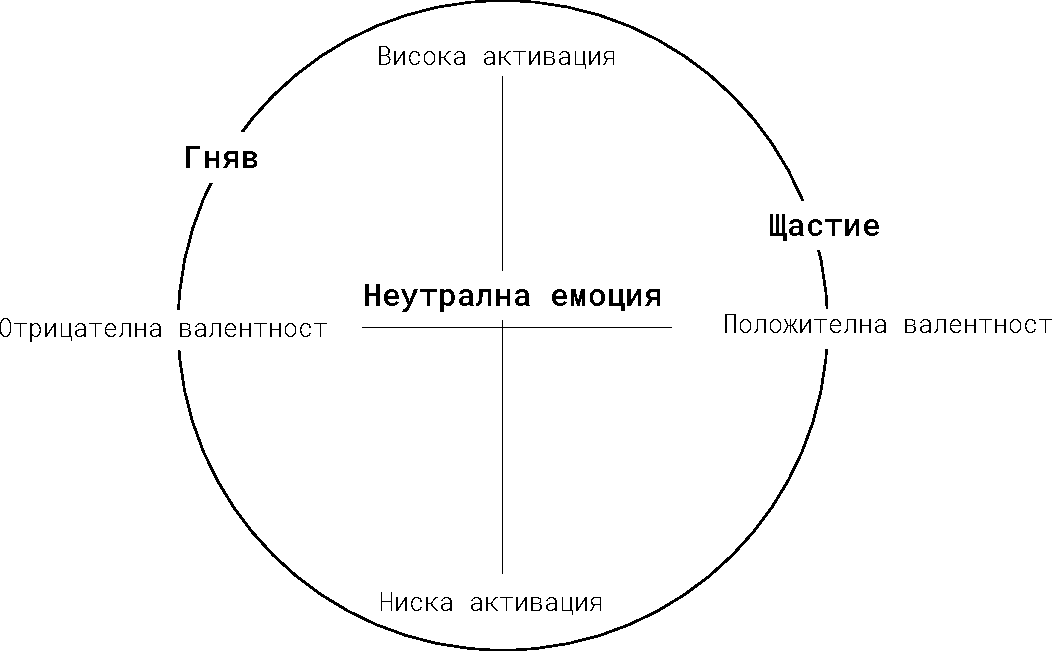
\includegraphics[width=\textwidth]{valence_arousal_ahn}%
                \end{center}
            \end{column}%
        \end{columns}
    \end{frame}


    \begin{frame}{Нулева зона (какво е емоция)}
        \begin{columns}[T] % align columns
            \begin{column}{.38\textwidth}
                \textbf{Избрани емоции:}
                \vspace{1cm}\\
                $\bullet\ $ Гняв
                \vspace{1cm}\\
                $\bullet\ $ Щастие
                \vspace{1cm}\\
                $\bullet\ $ Неутрална емоция
                \vspace{1cm}\\
                $\bullet\ $ Тъга
            \end{column}%
            \hfill%
            \begin{column}{.60\textwidth}
                \vspace{1cm}
                \begin{center}
                    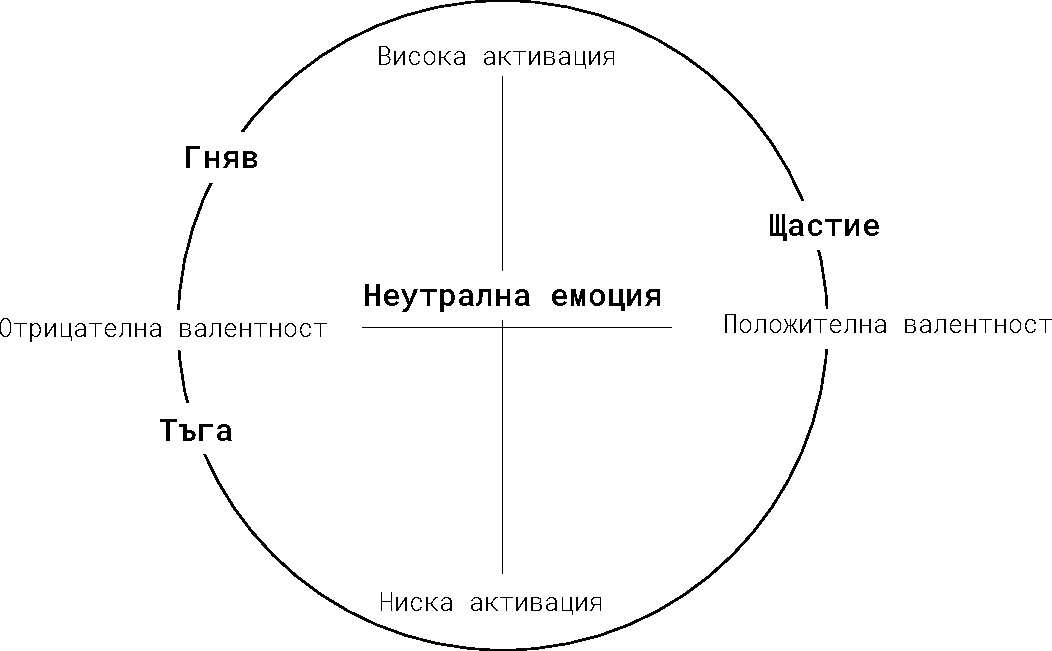
\includegraphics[width=\textwidth]{valence_arousal_ahns}%
                \end{center}
            \end{column}%
        \end{columns}
    \end{frame}

    \section{Сигнал от реч}

    \begin{frame}{Сигнал от реч}
        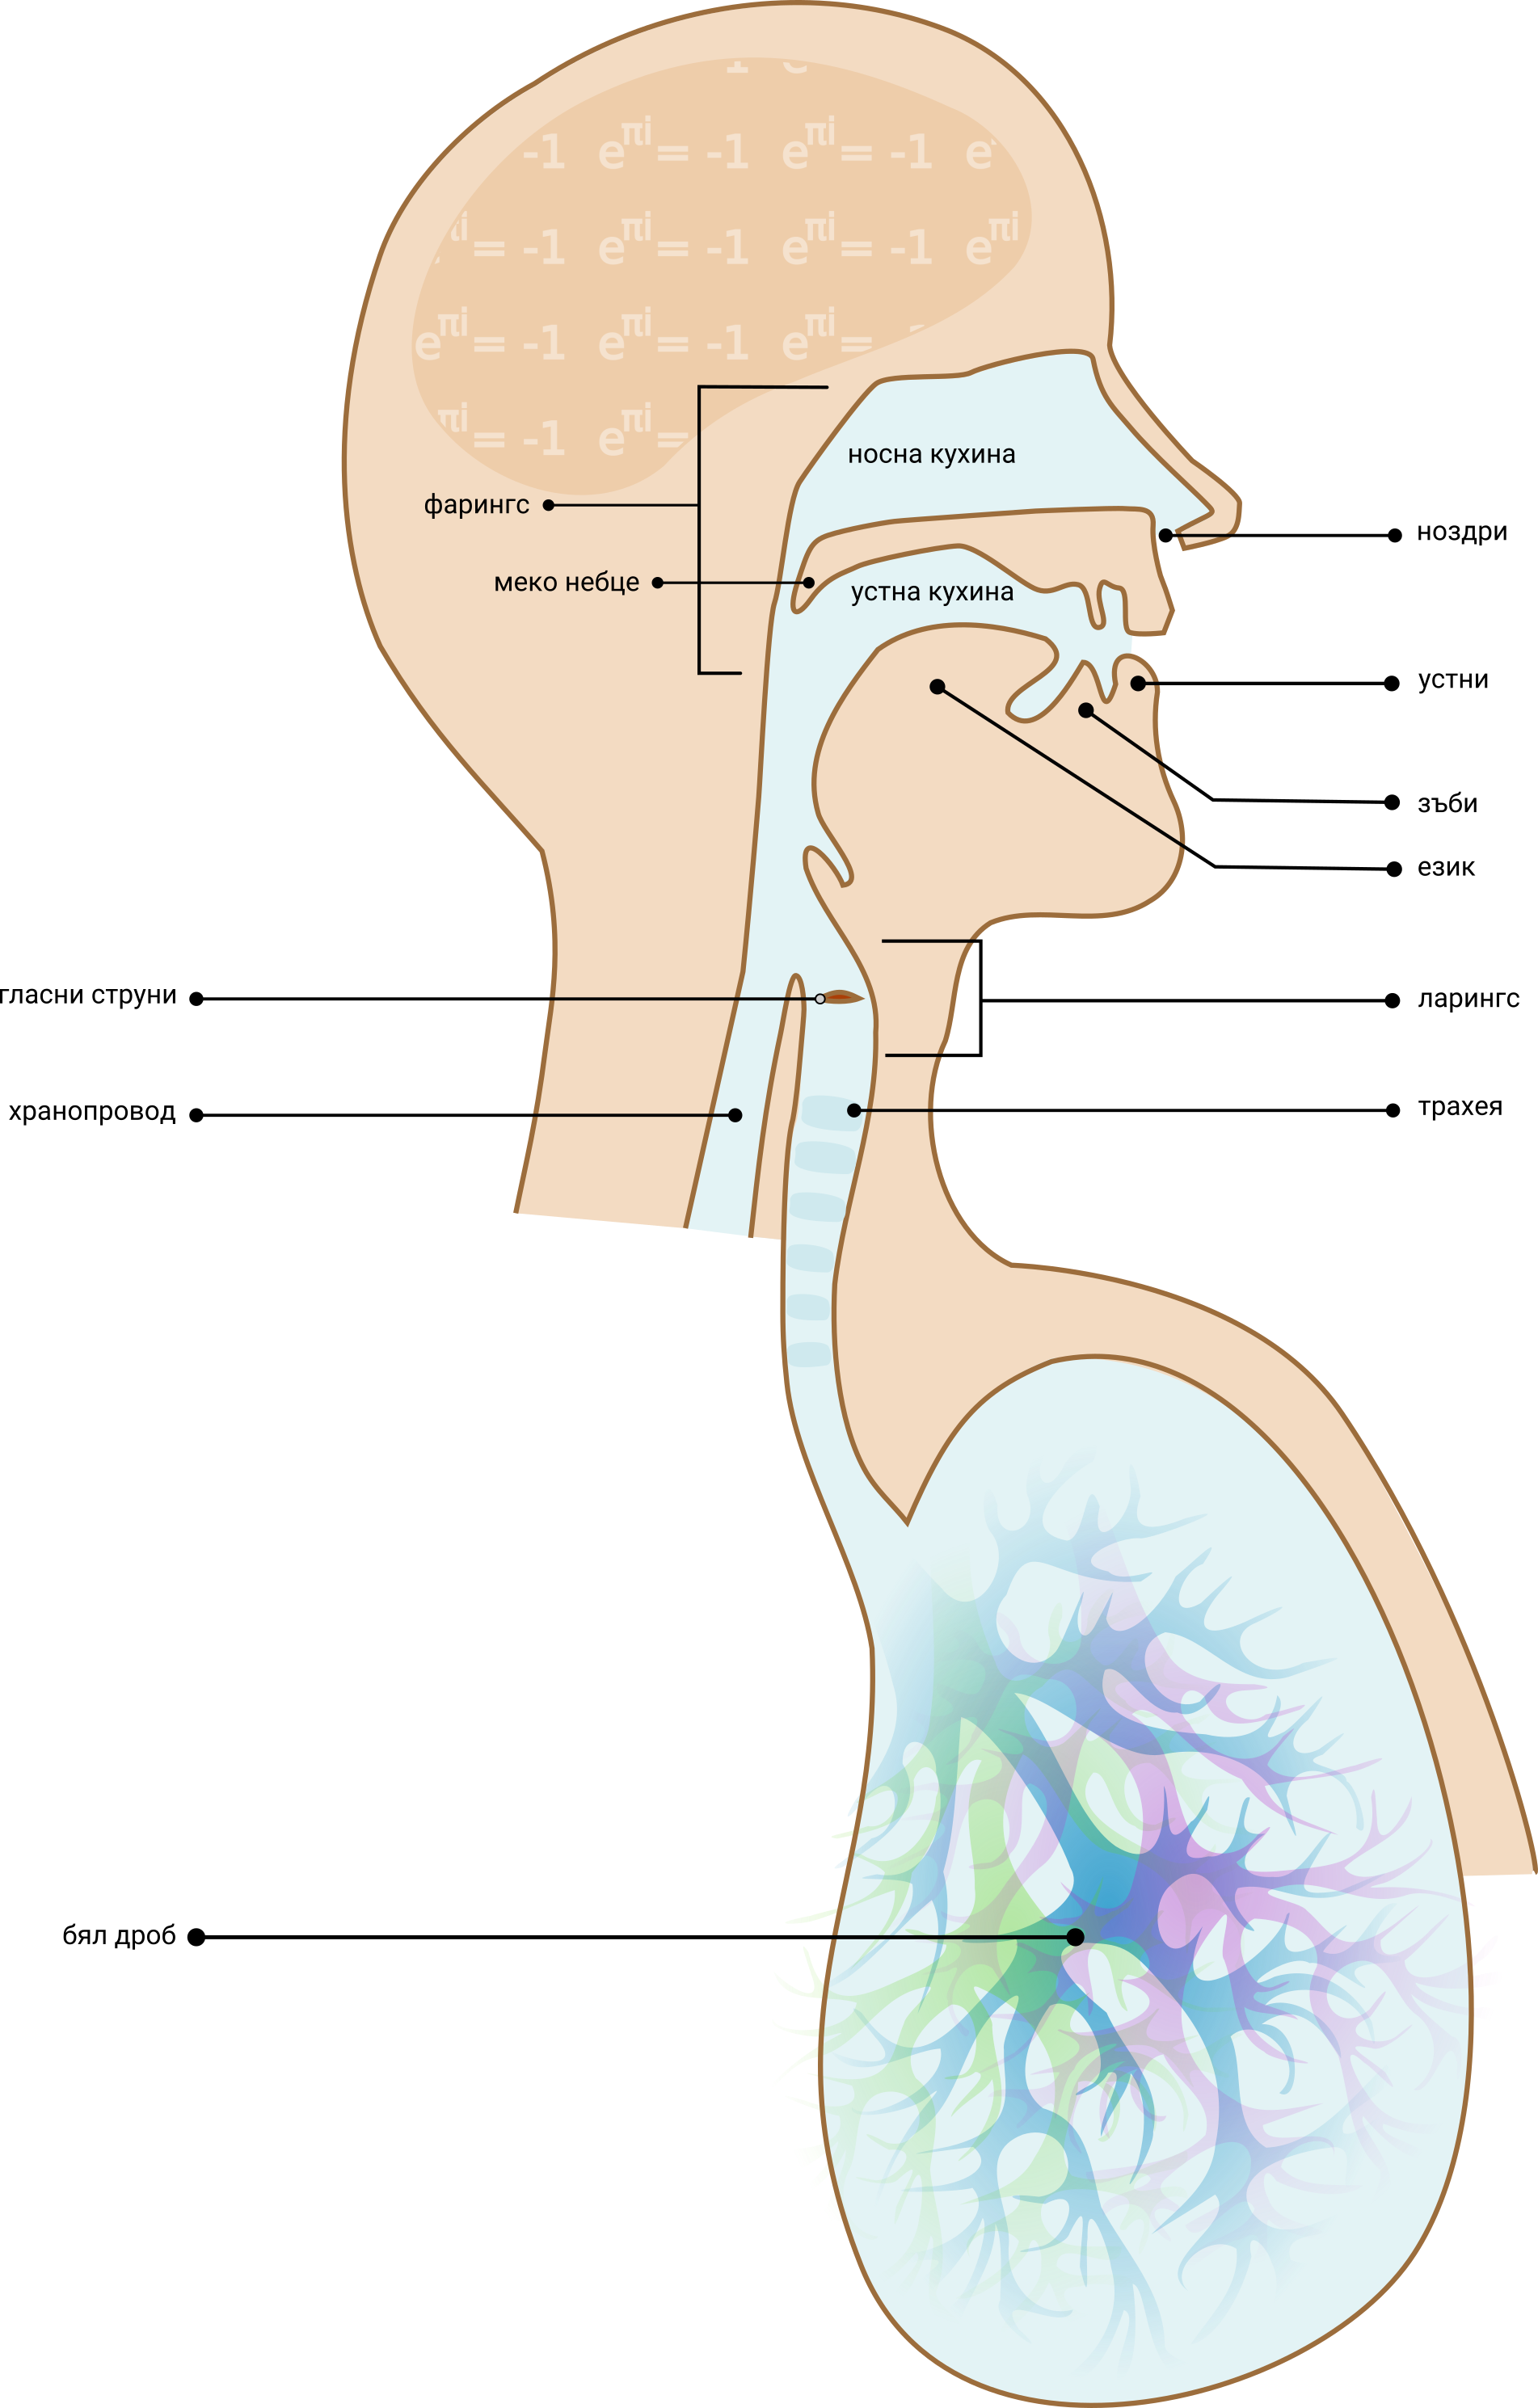
\includegraphics[width=0.48\paperwidth]{physics}%
        \hfill
        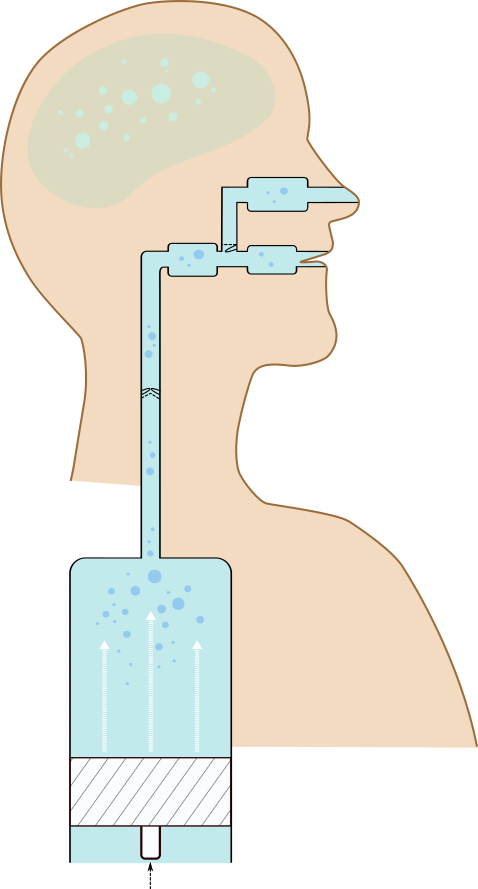
\includegraphics[width=0.28\paperwidth]{tubes}%
    \end{frame}

    \begin{frame}{Сигнал от реч}
        \centering{
            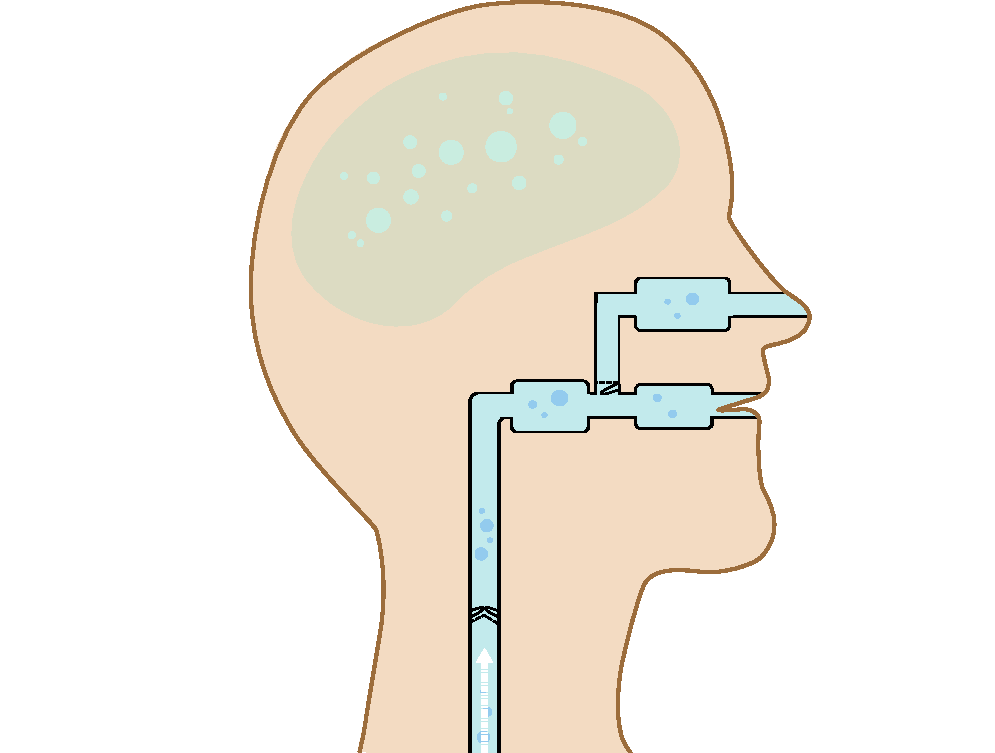
\includegraphics[height=\textheight]{glottis}%
        }
    \end{frame}

    \begin{frame}{Сигнал от реч}
    Видове звуци:
    \vspace{1cm}\\
    \pause
    \begin{itemize}
        \item Озвучени - ``а''
        \pause
        \item Проходни (фрикативни) - ``с''
        \pause
        \item Преградни - ``п'' 
    \end{itemize}
    \vspace{1cm}
    \pause
    Реч \pause$\rightarrow$ думи \pause $\rightarrow$ фонеми 
    \vspace{1cm}\\
    \pause
    ``Страхът стискаше гърлото, задушаваше гласа.''
    \end{frame}

    \begin{frame}{Сигнал от реч}
        \begin{itemize}
            \item Спектрални характеристики
            \pause
            \item Честотна пропускливост
        \end{itemize}
        \pause
        \centering{
            
\includegraphics[width=\textwidth]{trombone}%
        }
        \pause
        \textbf{За да изследваме подлежащата емоция, трябва да изследваме спектралните свойства на статична конфигурация на вокалния тракт.}
    \end{frame}

\end{document}